\section{Teilaufgabe 24}
\begin{aufgabe}
    Fügen Sie in Ihrem Simulink Progamm einen Saturation Block hinzu, sodass 
    die Eingangsspannung des Motors nur Werte zwischen -10 (V) und +10 (V) 
    annimmt.  Die Referenzdrehzahl sollte nach ungefähr 100 (ms) einen Sprung 
    von 50 auf 100 (rad/s) machen. Führen Sie ein paar Simulationen durch und 
    beobachten Sie die Eingangsspannung. Was passiert, wenn die Verstärkung 
    des Reglers gross wird.
\end{aufgabe}
\begin{figure}[h!]
    \centering
    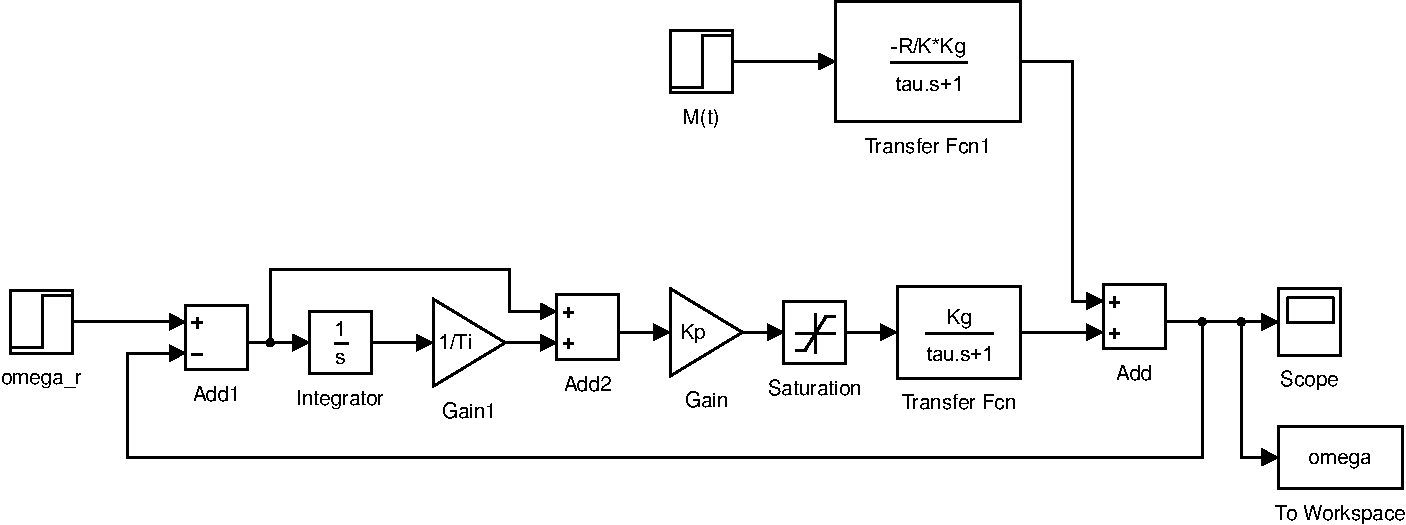
\includegraphics[width=0.6\textwidth]{24/regler_sat.pdf}
    \caption{Regler in Simulink}
    \label{fig:24}
\end{figure}
\begin{figure}[h!]
    \centering
    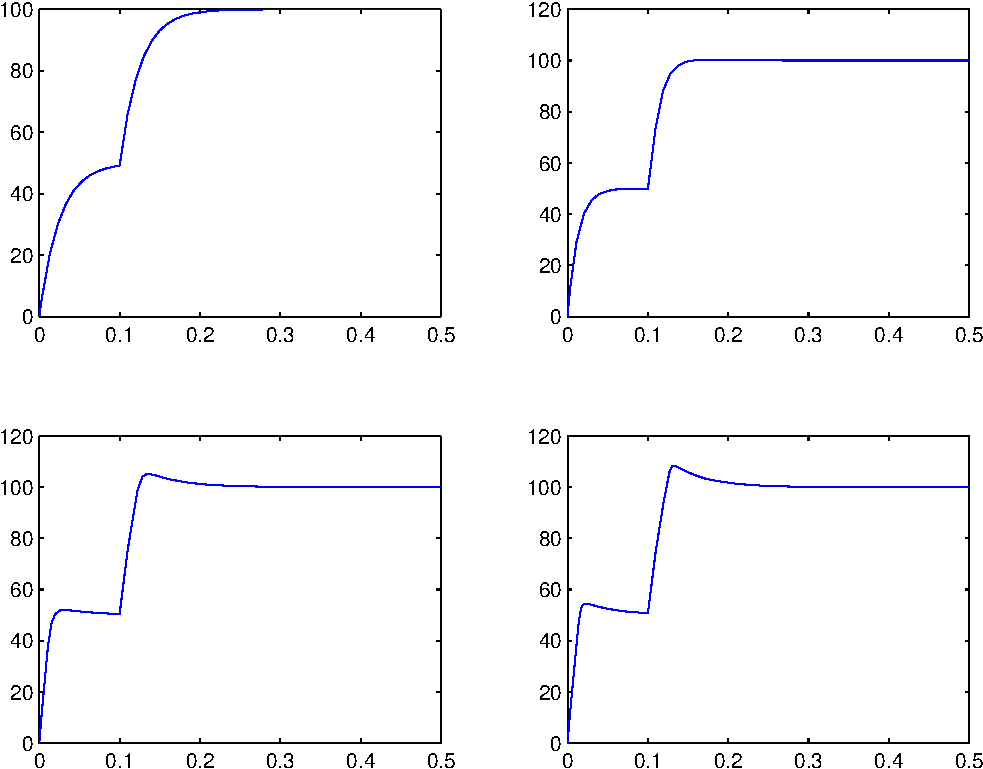
\includegraphics[width=0.6\textwidth]{24/regler_sat_plot.pdf}
    \caption{Simulationsergebnis}
    \label{fig:24plot}
\end{figure}
\lstinputlisting{24/regler_sat.m}
Wird die Verstärkung zu gross, beginnt die Sättigung zu wirken und der 
Integrator läuft davon. Dies ist deutlich am Überschwingen zu erkennen. 
